\documentclass[1p]{elsarticle_modified}
%\bibliographystyle{elsarticle-num}

%\usepackage[colorlinks]{hyperref}
%\usepackage{abbrmath_seonhwa} %\Abb, \Ascr, \Acal ,\Abf, \Afrak
\usepackage{amsfonts}
\usepackage{amssymb}
\usepackage{amsmath}
\usepackage{amsthm}
\usepackage{scalefnt}
\usepackage{amsbsy}
\usepackage{kotex}
\usepackage{caption}
\usepackage{subfig}
\usepackage{color}
\usepackage{graphicx}
\usepackage{xcolor} %% white, black, red, green, blue, cyan, magenta, yellow
\usepackage{float}
\usepackage{setspace}
\usepackage{hyperref}

\usepackage{tikz}
\usetikzlibrary{arrows}

\usepackage{multirow}
\usepackage{array} % fixed length table
\usepackage{hhline}

%%%%%%%%%%%%%%%%%%%%%
\makeatletter
\renewcommand*\env@matrix[1][\arraystretch]{%
	\edef\arraystretch{#1}%
	\hskip -\arraycolsep
	\let\@ifnextchar\new@ifnextchar
	\array{*\c@MaxMatrixCols c}}
\makeatother %https://tex.stackexchange.com/questions/14071/how-can-i-increase-the-line-spacing-in-a-matrix
%%%%%%%%%%%%%%%

\usepackage[normalem]{ulem}

\newcommand{\msout}[1]{\ifmmode\text{\sout{\ensuremath{#1}}}\else\sout{#1}\fi}
%SOURCE: \msout is \stkout macro in https://tex.stackexchange.com/questions/20609/strikeout-in-math-mode

\newcommand{\cancel}[1]{
	\ifmmode
	{\color{red}\msout{#1}}
	\else
	{\color{red}\sout{#1}}
	\fi
}

\newcommand{\add}[1]{
	{\color{blue}\uwave{#1}}
}

\newcommand{\replace}[2]{
	\ifmmode
	{\color{red}\msout{#1}}{\color{blue}\uwave{#2}}
	\else
	{\color{red}\sout{#1}}{\color{blue}\uwave{#2}}
	\fi
}

\newcommand{\Sol}{\mathcal{S}} %segment
\newcommand{\D}{D} %diagram
\newcommand{\A}{\mathcal{A}} %arc


%%%%%%%%%%%%%%%%%%%%%%%%%%%%%5 test

\def\sl{\operatorname{\textup{SL}}(2,\Cbb)}
\def\psl{\operatorname{\textup{PSL}}(2,\Cbb)}
\def\quan{\mkern 1mu \triangleright \mkern 1mu}

\theoremstyle{definition}
\newtheorem{thm}{Theorem}[section]
\newtheorem{prop}[thm]{Proposition}
\newtheorem{lem}[thm]{Lemma}
\newtheorem{ques}[thm]{Question}
\newtheorem{cor}[thm]{Corollary}
\newtheorem{defn}[thm]{Definition}
\newtheorem{exam}[thm]{Example}
\newtheorem{rmk}[thm]{Remark}
\newtheorem{alg}[thm]{Algorithm}

\newcommand{\I}{\sqrt{-1}}
\begin{document}

%\begin{frontmatter}
%
%\title{Boundary parabolic representations of knots up to 8 crossings}
%
%%% Group authors per affiliation:
%\author{Yunhi Cho} 
%\address{Department of Mathematics, University of Seoul, Seoul, Korea}
%\ead{yhcho@uos.ac.kr}
%
%
%\author{Seonhwa Kim} %\fnref{s_kim}}
%\address{Center for Geometry and Physics, Institute for Basic Science, Pohang, 37673, Korea}
%\ead{ryeona17@ibs.re.kr}
%
%\author{Hyuk Kim}
%\address{Department of Mathematical Sciences, Seoul National University, Seoul 08826, Korea}
%\ead{hyukkim@snu.ac.kr}
%
%\author{Seokbeom Yoon}
%\address{Department of Mathematical Sciences, Seoul National University, Seoul, 08826,  Korea}
%\ead{sbyoon15@snu.ac.kr}
%
%\begin{abstract}
%We find all boundary parabolic representation of knots up to 8 crossings.
%
%\end{abstract}
%\begin{keyword}
%    \MSC[2010] 57M25 
%\end{keyword}
%
%\end{frontmatter}

%\linenumbers
%\tableofcontents
%
\newcommand\colored[1]{\textcolor{white}{\rule[-0.35ex]{0.8em}{1.4ex}}\kern-0.8em\color{red} #1}%
%\newcommand\colored[1]{\textcolor{white}{ #1}\kern-2.17ex	\textcolor{white}{ #1}\kern-1.81ex	\textcolor{white}{ #1}\kern-2.15ex\color{red}#1	}

{\Large $\underline{12n_{0217}~(K12n_{0217})}$}

\setlength{\tabcolsep}{10pt}
\renewcommand{\arraystretch}{1.6}
\vspace{1cm}\begin{tabular}{m{100pt}>{\centering\arraybackslash}m{274pt}}
\multirow{5}{120pt}{
	\centering
	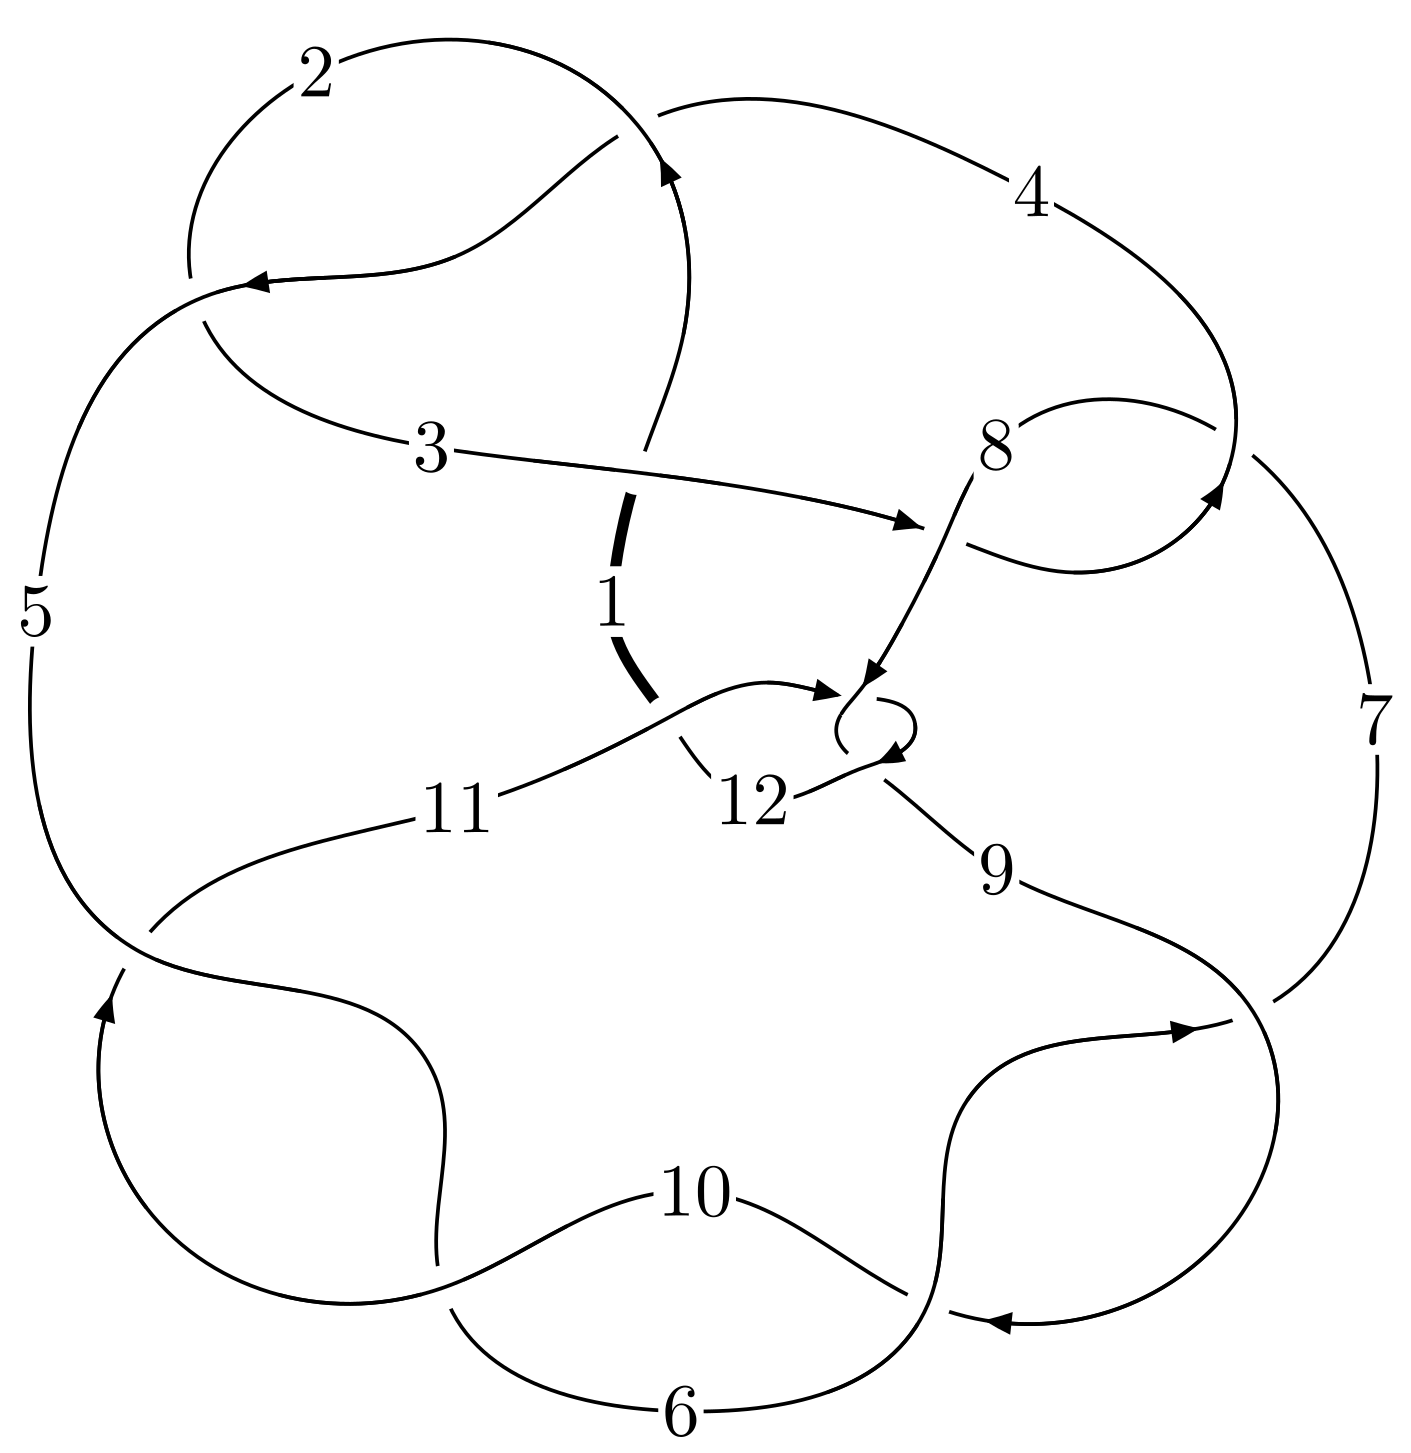
\includegraphics[width=112pt]{../../../GIT/diagram.site/Diagrams/png/2306_12n_0217.png}\\
\ \ \ A knot diagram\footnotemark}&
\allowdisplaybreaks
\textbf{Linearized knot diagam} \\
\cline{2-2}
 &
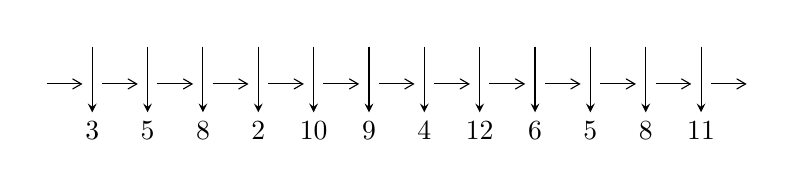
\begin{tikzpicture}[x=20pt, y=17pt]
	% nodes
	\node (C0) at (0, 0) {};
	\node (C1) at (1, 0) {};
	\node (C1U) at (1, +1) {};
	\node (C1D) at (1, -1) {3};

	\node (C2) at (2, 0) {};
	\node (C2U) at (2, +1) {};
	\node (C2D) at (2, -1) {5};

	\node (C3) at (3, 0) {};
	\node (C3U) at (3, +1) {};
	\node (C3D) at (3, -1) {8};

	\node (C4) at (4, 0) {};
	\node (C4U) at (4, +1) {};
	\node (C4D) at (4, -1) {2};

	\node (C5) at (5, 0) {};
	\node (C5U) at (5, +1) {};
	\node (C5D) at (5, -1) {10};

	\node (C6) at (6, 0) {};
	\node (C6U) at (6, +1) {};
	\node (C6D) at (6, -1) {9};

	\node (C7) at (7, 0) {};
	\node (C7U) at (7, +1) {};
	\node (C7D) at (7, -1) {4};

	\node (C8) at (8, 0) {};
	\node (C8U) at (8, +1) {};
	\node (C8D) at (8, -1) {12};

	\node (C9) at (9, 0) {};
	\node (C9U) at (9, +1) {};
	\node (C9D) at (9, -1) {6};

	\node (C10) at (10, 0) {};
	\node (C10U) at (10, +1) {};
	\node (C10D) at (10, -1) {5};

	\node (C11) at (11, 0) {};
	\node (C11U) at (11, +1) {};
	\node (C11D) at (11, -1) {8};

	\node (C12) at (12, 0) {};
	\node (C12U) at (12, +1) {};
	\node (C12D) at (12, -1) {11};
	\node (C13) at (13, 0) {};

	% arrows
	\draw[->,>={angle 60}]
	(C0) edge (C1) (C1) edge (C2) (C2) edge (C3) (C3) edge (C4) (C4) edge (C5) (C5) edge (C6) (C6) edge (C7) (C7) edge (C8) (C8) edge (C9) (C9) edge (C10) (C10) edge (C11) (C11) edge (C12) (C12) edge (C13) ;	\draw[->,>=stealth]
	(C1U) edge (C1D) (C2U) edge (C2D) (C3U) edge (C3D) (C4U) edge (C4D) (C5U) edge (C5D) (C6U) edge (C6D) (C7U) edge (C7D) (C8U) edge (C8D) (C9U) edge (C9D) (C10U) edge (C10D) (C11U) edge (C11D) (C12U) edge (C12D) ;
	\end{tikzpicture} \\
\hhline{~~} \\& 
\textbf{Solving Sequence} \\ \cline{2-2} 
 &
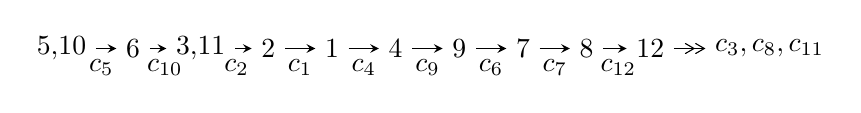
\begin{tikzpicture}[x=23pt, y=7pt]
	% node
	\node (A0) at (-1/8, 0) {5,10};
	\node (A1) at (1, 0) {6};
	\node (A2) at (33/16, 0) {3,11};
	\node (A3) at (25/8, 0) {2};
	\node (A4) at (33/8, 0) {1};
	\node (A5) at (41/8, 0) {4};
	\node (A6) at (49/8, 0) {9};
	\node (A7) at (57/8, 0) {7};
	\node (A8) at (65/8, 0) {8};
	\node (A9) at (73/8, 0) {12};
	\node (C1) at (1/2, -1) {$c_{5}$};
	\node (C2) at (3/2, -1) {$c_{10}$};
	\node (C3) at (21/8, -1) {$c_{2}$};
	\node (C4) at (29/8, -1) {$c_{1}$};
	\node (C5) at (37/8, -1) {$c_{4}$};
	\node (C6) at (45/8, -1) {$c_{9}$};
	\node (C7) at (53/8, -1) {$c_{6}$};
	\node (C8) at (61/8, -1) {$c_{7}$};
	\node (C9) at (69/8, -1) {$c_{12}$};
	\node (A10) at (11, 0) {$c_{3},c_{8},c_{11}$};

	% edge
	\draw[->,>=stealth]	
	(A0) edge (A1) (A1) edge (A2) (A2) edge (A3) (A3) edge (A4) (A4) edge (A5) (A5) edge (A6) (A6) edge (A7) (A7) edge (A8) (A8) edge (A9) ;
	\draw[->>,>={angle 60}]	
	(A9) edge (A10);
\end{tikzpicture} \\ 

\end{tabular} \\

\footnotetext{
The image of knot diagram is generated by the software ``\textbf{Draw programme}" developed by Andrew Bartholomew(\url{http://www.layer8.co.uk/maths/draw/index.htm\#Running-draw}), where we modified some parts for our purpose(\url{https://github.com/CATsTAILs/LinksPainter}).
}\phantom \\ \newline 
\centering \textbf{Ideals for irreducible components\footnotemark of $X_{\text{par}}$} 
 
\begin{align*}
I^u_{1}&=\langle 
-701858710240 u^{15}+1651068868988 u^{14}+\cdots+11848301554132 b+11254876138420,\\
\phantom{I^u_{1}}&\phantom{= \langle  }11529472260049 u^{15}-21953100573652 u^{14}+\cdots+71089809324792 a+197556161100296,\\
\phantom{I^u_{1}}&\phantom{= \langle  }u^{16}-2 u^{15}+\cdots-8 u-8\rangle \\
I^u_{2}&=\langle 
b+1,\;4 u^4-3 u^3+16 u^2+3 a-8 u+10,\;u^5- u^4+4 u^3-3 u^2+3 u-1\rangle \\
I^u_{3}&=\langle 
-32 a^2 u-18 a^2+10 a u+593 b+228 a-70 u-410,\;4 a^3-6 a^2 u-4 a^2-8 a u-8 a- u-36,\;u^2+2\rangle \\
\\
I^v_{1}&=\langle 
a,\;- v^2+b-3 v+1,\;v^3+2 v^2-3 v+1\rangle \\
\end{align*}
\raggedright * 4 irreducible components of $\dim_{\mathbb{C}}=0$, with total 30 representations.\\
\footnotetext{All coefficients of polynomials are rational numbers. But the coefficients are sometimes approximated in decimal forms when there is not enough margin.}
\newpage
\renewcommand{\arraystretch}{1}
\centering \section*{I. $I^u_{1}= \langle -7.02\times10^{11} u^{15}+1.65\times10^{12} u^{14}+\cdots+1.18\times10^{13} b+1.13\times10^{13},\;1.15\times10^{13} u^{15}-2.20\times10^{13} u^{14}+\cdots+7.11\times10^{13} a+1.98\times10^{14},\;u^{16}-2 u^{15}+\cdots-8 u-8 \rangle$}
\flushleft \textbf{(i) Arc colorings}\\
\begin{tabular}{m{7pt} m{180pt} m{7pt} m{180pt} }
\flushright $a_{5}=$&$\begin{pmatrix}1\\0\end{pmatrix}$ \\
\flushright $a_{10}=$&$\begin{pmatrix}0\\u\end{pmatrix}$ \\
\flushright $a_{6}=$&$\begin{pmatrix}1\\u^2\end{pmatrix}$ \\
\flushright $a_{3}=$&$\begin{pmatrix}-0.162182 u^{15}+0.308808 u^{14}+\cdots-20.6422 u-2.77897\\0.0592371 u^{15}-0.139351 u^{14}+\cdots-1.86827 u-0.949915\end{pmatrix}$ \\
\flushright $a_{11}=$&$\begin{pmatrix}- u\\u\end{pmatrix}$ \\
\flushright $a_{2}=$&$\begin{pmatrix}-0.102945 u^{15}+0.169457 u^{14}+\cdots-22.5104 u-3.72888\\0.0592371 u^{15}-0.139351 u^{14}+\cdots-1.86827 u-0.949915\end{pmatrix}$ \\
\flushright $a_{1}=$&$\begin{pmatrix}-0.0354092 u^{15}+0.0455388 u^{14}+\cdots-6.52383 u-0.485363\\0.0593874 u^{15}-0.138415 u^{14}+\cdots-0.826057 u-0.465521\end{pmatrix}$ \\
\flushright $a_{4}=$&$\begin{pmatrix}-0.152070 u^{15}+0.290947 u^{14}+\cdots-18.3389 u-2.21890\\0.000477366 u^{15}-0.0269082 u^{14}+\cdots-1.35512 u+0.0663976\end{pmatrix}$ \\
\flushright $a_{9}=$&$\begin{pmatrix}u\\u^3+u\end{pmatrix}$ \\
\flushright $a_{7}=$&$\begin{pmatrix}u^2+1\\u^4+2 u^2\end{pmatrix}$ \\
\flushright $a_{8}=$&$\begin{pmatrix}-0.0357612 u^{15}+0.0641648 u^{14}+\cdots-6.69137 u-0.844724\\-0.0626778 u^{15}+0.160544 u^{14}+\cdots+0.313570 u+0.0472977\end{pmatrix}$ \\
\flushright $a_{12}=$&$\begin{pmatrix}-0.0357612 u^{15}+0.0641648 u^{14}+\cdots-6.69137 u-0.844724\\0.0597395 u^{15}-0.157041 u^{14}+\cdots-0.658521 u-0.106159\end{pmatrix}$\\&\end{tabular}
\flushleft \textbf{(ii) Obstruction class $= -1$}\\~\\
\flushleft \textbf{(iii) Cusp Shapes $= -\frac{1637037920523}{11848301554132} u^{15}+\frac{2186962426267}{8886226165599} u^{14}+\cdots-\frac{226259574309964}{2962075388533} u-\frac{279610162162742}{8886226165599}$}\\~\\
\newpage\renewcommand{\arraystretch}{1}
\flushleft \textbf{(iv) u-Polynomials at the component}\newline \\
\begin{tabular}{m{50pt}|m{274pt}}
Crossings & \hspace{64pt}u-Polynomials at each crossing \\
\hline $$\begin{aligned}c_{1}\end{aligned}$$&$\begin{aligned}
&u^{16}-5 u^{15}+\cdots+2230 u+81
\end{aligned}$\\
\hline $$\begin{aligned}c_{2},c_{4}\end{aligned}$$&$\begin{aligned}
&u^{16}-9 u^{15}+\cdots+40 u+9
\end{aligned}$\\
\hline $$\begin{aligned}c_{3},c_{7}\end{aligned}$$&$\begin{aligned}
&u^{16}+2 u^{15}+\cdots+192 u-288
\end{aligned}$\\
\hline $$\begin{aligned}c_{5},c_{6},c_{9}\\c_{10}\end{aligned}$$&$\begin{aligned}
&u^{16}-2 u^{15}+\cdots-8 u-8
\end{aligned}$\\
\hline $$\begin{aligned}c_{8},c_{11}\end{aligned}$$&$\begin{aligned}
&u^{16}+5 u^{15}+\cdots+77 u+49
\end{aligned}$\\
\hline $$\begin{aligned}c_{12}\end{aligned}$$&$\begin{aligned}
&u^{16}-7 u^{15}+\cdots+11515 u+2401
\end{aligned}$\\
\hline
\end{tabular}\\~\\
\newpage\renewcommand{\arraystretch}{1}
\flushleft \textbf{(v) Riley Polynomials at the component}\newline \\
\begin{tabular}{m{50pt}|m{274pt}}
Crossings & \hspace{64pt}Riley Polynomials at each crossing \\
\hline $$\begin{aligned}c_{1}\end{aligned}$$&$\begin{aligned}
&y^{16}+125 y^{15}+\cdots-5228050 y+6561
\end{aligned}$\\
\hline $$\begin{aligned}c_{2},c_{4}\end{aligned}$$&$\begin{aligned}
&y^{16}+5 y^{15}+\cdots-2230 y+81
\end{aligned}$\\
\hline $$\begin{aligned}c_{3},c_{7}\end{aligned}$$&$\begin{aligned}
&y^{16}+78 y^{15}+\cdots-935424 y+82944
\end{aligned}$\\
\hline $$\begin{aligned}c_{5},c_{6},c_{9}\\c_{10}\end{aligned}$$&$\begin{aligned}
&y^{16}+32 y^{15}+\cdots-1216 y+64
\end{aligned}$\\
\hline $$\begin{aligned}c_{8},c_{11}\end{aligned}$$&$\begin{aligned}
&y^{16}+7 y^{15}+\cdots-11515 y+2401
\end{aligned}$\\
\hline $$\begin{aligned}c_{12}\end{aligned}$$&$\begin{aligned}
&y^{16}+223 y^{15}+\cdots-218306123 y+5764801
\end{aligned}$\\
\hline
\end{tabular}\\~\\
\newpage\flushleft \textbf{(vi) Complex Volumes and Cusp Shapes}
$$\begin{array}{c|c|c}  
\text{Solutions to }I^u_{1}& \I (\text{vol} + \sqrt{-1}CS) & \text{Cusp shape}\\
 \hline 
\begin{aligned}
u &= \phantom{-}0.010246 + 1.149370 I \\
a &= \phantom{-}0.791080 - 0.938892 I \\
b &= -0.214689 + 0.526707 I\end{aligned}
 & \phantom{-}2.75443 + 1.56440 I & -5.92206 - 4.42049 I \\ \hline\begin{aligned}
u &= \phantom{-}0.010246 - 1.149370 I \\
a &= \phantom{-}0.791080 + 0.938892 I \\
b &= -0.214689 - 0.526707 I\end{aligned}
 & \phantom{-}2.75443 - 1.56440 I & -5.92206 + 4.42049 I \\ \hline\begin{aligned}
u &= -0.523193 + 0.477390 I \\
a &= \phantom{-}0.845221 + 0.799076 I \\
b &= -0.840636 - 0.527182 I\end{aligned}
 & -0.699414 - 0.322898 I & -10.19188 - 0.54504 I \\ \hline\begin{aligned}
u &= -0.523193 - 0.477390 I \\
a &= \phantom{-}0.845221 - 0.799076 I \\
b &= -0.840636 + 0.527182 I\end{aligned}
 & -0.699414 + 0.322898 I & -10.19188 + 0.54504 I \\ \hline\begin{aligned}
u &= -0.307601 + 0.557834 I \\
a &= \phantom{-}0.369622 + 0.769525 I \\
b &= \phantom{-}0.719726 - 0.602269 I\end{aligned}
 & \phantom{-}1.30361 + 3.67873 I & -7.60649 - 8.93405 I \\ \hline\begin{aligned}
u &= -0.307601 - 0.557834 I \\
a &= \phantom{-}0.369622 - 0.769525 I \\
b &= \phantom{-}0.719726 + 0.602269 I\end{aligned}
 & \phantom{-}1.30361 - 3.67873 I & -7.60649 + 8.93405 I \\ \hline\begin{aligned}
u &= -0.398844\phantom{ +0.000000I} \\
a &= \phantom{-}0.830482\phantom{ +0.000000I} \\
b &= -0.188115\phantom{ +0.000000I}\end{aligned}
 & -0.713389\phantom{ +0.000000I} & -13.5530\phantom{ +0.000000I} \\ \hline\begin{aligned}
u &= \phantom{-}0.02902 + 1.65352 I \\
a &= -0.817077 + 0.790518 I \\
b &= \phantom{-}1.069770 - 0.413434 I\end{aligned}
 & \phantom{-}9.00996 + 4.18278 I & -7.18732 - 6.68831 I \\ \hline\begin{aligned}
u &= \phantom{-}0.02902 - 1.65352 I \\
a &= -0.817077 - 0.790518 I \\
b &= \phantom{-}1.069770 + 0.413434 I\end{aligned}
 & \phantom{-}9.00996 - 4.18278 I & -7.18732 + 6.68831 I \\ \hline\begin{aligned}
u &= \phantom{-}0.234441\phantom{ +0.000000I} \\
a &= -12.8312\phantom{ +0.000000I} \\
b &= -0.889606\phantom{ +0.000000I}\end{aligned}
 & -2.92059\phantom{ +0.000000I} & -60.0340\phantom{ +0.000000I}\\
 \hline 
 \end{array}$$\newpage$$\begin{array}{c|c|c}  
\text{Solutions to }I^u_{1}& \I (\text{vol} + \sqrt{-1}CS) & \text{Cusp shape}\\
 \hline 
\begin{aligned}
u &= \phantom{-}0.42095 + 1.83693 I \\
a &= -1.25179 - 2.08277 I \\
b &= \phantom{-}1.56472 + 0.94125 I\end{aligned}
 & -14.6966 - 11.6900 I & -9.38618 + 4.27031 I \\ \hline\begin{aligned}
u &= \phantom{-}0.42095 - 1.83693 I \\
a &= -1.25179 + 2.08277 I \\
b &= \phantom{-}1.56472 - 0.94125 I\end{aligned}
 & -14.6966 + 11.6900 I & -9.38618 - 4.27031 I \\ \hline\begin{aligned}
u &= \phantom{-}1.17925 + 1.85135 I \\
a &= -0.79943 - 2.75277 I \\
b &= \phantom{-}1.31233 + 2.03102 I\end{aligned}
 & \phantom{-}14.0944 - 4.3162 I & -8.81389 + 1.69710 I \\ \hline\begin{aligned}
u &= \phantom{-}1.17925 - 1.85135 I \\
a &= -0.79943 + 2.75277 I \\
b &= \phantom{-}1.31233 - 2.03102 I\end{aligned}
 & \phantom{-}14.0944 + 4.3162 I & -8.81389 - 1.69710 I \\ \hline\begin{aligned}
u &= \phantom{-}0.27353 + 2.59286 I \\
a &= -1.63728 + 2.97926 I \\
b &= \phantom{-}1.42763 - 2.33180 I\end{aligned}
 & -11.59440 - 0.80168 I & -8.76521 + 0.15055 I \\ \hline\begin{aligned}
u &= \phantom{-}0.27353 - 2.59286 I \\
a &= -1.63728 - 2.97926 I \\
b &= \phantom{-}1.42763 + 2.33180 I\end{aligned}
 & -11.59440 + 0.80168 I & -8.76521 - 0.15055 I\\
 \hline 
 \end{array}$$\newpage\newpage\renewcommand{\arraystretch}{1}
\centering \section*{II. $I^u_{2}= \langle b+1,\;4 u^4-3 u^3+16 u^2+3 a-8 u+10,\;u^5- u^4+4 u^3-3 u^2+3 u-1 \rangle$}
\flushleft \textbf{(i) Arc colorings}\\
\begin{tabular}{m{7pt} m{180pt} m{7pt} m{180pt} }
\flushright $a_{5}=$&$\begin{pmatrix}1\\0\end{pmatrix}$ \\
\flushright $a_{10}=$&$\begin{pmatrix}0\\u\end{pmatrix}$ \\
\flushright $a_{6}=$&$\begin{pmatrix}1\\u^2\end{pmatrix}$ \\
\flushright $a_{3}=$&$\begin{pmatrix}-\frac{4}{3} u^4+u^3+\cdots+\frac{8}{3} u-\frac{10}{3}\\-1\end{pmatrix}$ \\
\flushright $a_{11}=$&$\begin{pmatrix}- u\\u\end{pmatrix}$ \\
\flushright $a_{2}=$&$\begin{pmatrix}-\frac{4}{3} u^4+u^3+\cdots+\frac{8}{3} u-\frac{13}{3}\\-1\end{pmatrix}$ \\
\flushright $a_{1}=$&$\begin{pmatrix}-1\\0\end{pmatrix}$ \\
\flushright $a_{4}=$&$\begin{pmatrix}-\frac{4}{3} u^4+u^3+\cdots+\frac{8}{3} u-\frac{10}{3}\\-1\end{pmatrix}$ \\
\flushright $a_{9}=$&$\begin{pmatrix}u\\u^3+u\end{pmatrix}$ \\
\flushright $a_{7}=$&$\begin{pmatrix}u^2+1\\u^4+2 u^2\end{pmatrix}$ \\
\flushright $a_{8}=$&$\begin{pmatrix}u^2+1\\u^4+2 u^2\end{pmatrix}$ \\
\flushright $a_{12}=$&$\begin{pmatrix}- u^2-1\\u^2\end{pmatrix}$\\&\end{tabular}
\flushleft \textbf{(ii) Obstruction class $= 1$}\\~\\
\flushleft \textbf{(iii) Cusp Shapes $= -\frac{14}{9} u^4+\frac{11}{3} u^3-\frac{77}{9} u^2+\frac{88}{9} u-\frac{137}{9}$}\\~\\
\newpage\renewcommand{\arraystretch}{1}
\flushleft \textbf{(iv) u-Polynomials at the component}\newline \\
\begin{tabular}{m{50pt}|m{274pt}}
Crossings & \hspace{64pt}u-Polynomials at each crossing \\
\hline $$\begin{aligned}c_{1},c_{2}\end{aligned}$$&$\begin{aligned}
&(u-1)^5
\end{aligned}$\\
\hline $$\begin{aligned}c_{3},c_{7}\end{aligned}$$&$\begin{aligned}
&u^5
\end{aligned}$\\
\hline $$\begin{aligned}c_{4}\end{aligned}$$&$\begin{aligned}
&(u+1)^5
\end{aligned}$\\
\hline $$\begin{aligned}c_{5},c_{6}\end{aligned}$$&$\begin{aligned}
&u^5- u^4+4 u^3-3 u^2+3 u-1
\end{aligned}$\\
\hline $$\begin{aligned}c_{8}\end{aligned}$$&$\begin{aligned}
&u^5- u^4+u^2+u-1
\end{aligned}$\\
\hline $$\begin{aligned}c_{9},c_{10},c_{12}\end{aligned}$$&$\begin{aligned}
&u^5+u^4+4 u^3+3 u^2+3 u+1
\end{aligned}$\\
\hline $$\begin{aligned}c_{11}\end{aligned}$$&$\begin{aligned}
&u^5+u^4- u^2+u+1
\end{aligned}$\\
\hline
\end{tabular}\\~\\
\newpage\renewcommand{\arraystretch}{1}
\flushleft \textbf{(v) Riley Polynomials at the component}\newline \\
\begin{tabular}{m{50pt}|m{274pt}}
Crossings & \hspace{64pt}Riley Polynomials at each crossing \\
\hline $$\begin{aligned}c_{1},c_{2},c_{4}\end{aligned}$$&$\begin{aligned}
&(y-1)^5
\end{aligned}$\\
\hline $$\begin{aligned}c_{3},c_{7}\end{aligned}$$&$\begin{aligned}
&y^5
\end{aligned}$\\
\hline $$\begin{aligned}c_{5},c_{6},c_{9}\\c_{10},c_{12}\end{aligned}$$&$\begin{aligned}
&y^5+7 y^4+16 y^3+13 y^2+3 y-1
\end{aligned}$\\
\hline $$\begin{aligned}c_{8},c_{11}\end{aligned}$$&$\begin{aligned}
&y^5- y^4+4 y^3-3 y^2+3 y-1
\end{aligned}$\\
\hline
\end{tabular}\\~\\
\newpage\flushleft \textbf{(vi) Complex Volumes and Cusp Shapes}
$$\begin{array}{c|c|c}  
\text{Solutions to }I^u_{2}& \I (\text{vol} + \sqrt{-1}CS) & \text{Cusp shape}\\
 \hline 
\begin{aligned}
u &= \phantom{-}0.233677 + 0.885557 I \\
a &= \phantom{-}0.162657 + 0.410020 I \\
b &= -1.00000\phantom{ +0.000000I}\end{aligned}
 & \phantom{-}0.17487 - 2.21397 I & -9.22580 + 4.04289 I \\ \hline\begin{aligned}
u &= \phantom{-}0.233677 - 0.885557 I \\
a &= \phantom{-}0.162657 - 0.410020 I \\
b &= -1.00000\phantom{ +0.000000I}\end{aligned}
 & \phantom{-}0.17487 + 2.21397 I & -9.22580 - 4.04289 I \\ \hline\begin{aligned}
u &= \phantom{-}0.416284\phantom{ +0.000000I} \\
a &= -3.11537\phantom{ +0.000000I} \\
b &= -1.00000\phantom{ +0.000000I}\end{aligned}
 & -2.52712\phantom{ +0.000000I} & -12.4170\phantom{ +0.000000I} \\ \hline\begin{aligned}
u &= \phantom{-}0.05818 + 1.69128 I \\
a &= \phantom{-}0.728361 + 0.139255 I \\
b &= -1.00000\phantom{ +0.000000I}\end{aligned}
 & \phantom{-}9.31336 - 3.33174 I & -4.67696 - 1.07305 I \\ \hline\begin{aligned}
u &= \phantom{-}0.05818 - 1.69128 I \\
a &= \phantom{-}0.728361 - 0.139255 I \\
b &= -1.00000\phantom{ +0.000000I}\end{aligned}
 & \phantom{-}9.31336 + 3.33174 I & -4.67696 + 1.07305 I\\
 \hline 
 \end{array}$$\newpage\newpage\renewcommand{\arraystretch}{1}
\centering \section*{III. $I^u_{3}= \langle -32 a^2 u+10 a u+\cdots+228 a-410,\;4 a^3-6 a^2 u-4 a^2-8 a u-8 a- u-36,\;u^2+2 \rangle$}
\flushleft \textbf{(i) Arc colorings}\\
\begin{tabular}{m{7pt} m{180pt} m{7pt} m{180pt} }
\flushright $a_{5}=$&$\begin{pmatrix}1\\0\end{pmatrix}$ \\
\flushright $a_{10}=$&$\begin{pmatrix}0\\u\end{pmatrix}$ \\
\flushright $a_{6}=$&$\begin{pmatrix}1\\-2\end{pmatrix}$ \\
\flushright $a_{3}=$&$\begin{pmatrix}a\\0.0539629 a^{2} u-0.0168634 a u+\cdots-0.384486 a+0.691400\end{pmatrix}$ \\
\flushright $a_{11}=$&$\begin{pmatrix}- u\\u\end{pmatrix}$ \\
\flushright $a_{2}=$&$\begin{pmatrix}0.0539629 a^{2} u-0.0168634 a u+\cdots+0.615514 a+0.691400\\0.0539629 a^{2} u-0.0168634 a u+\cdots-0.384486 a+0.691400\end{pmatrix}$ \\
\flushright $a_{1}=$&$\begin{pmatrix}-0.0607083 a^{2} u-0.231029 a u+\cdots-0.0674536 a-1.52782\\0.0607083 a^{2} u+0.231029 a u+\cdots+0.0674536 a+1.52782\end{pmatrix}$ \\
\flushright $a_{4}=$&$\begin{pmatrix}-0.0758853 a^{2} u-0.0387858 a u+\cdots-0.0843170 a+0.590219\\0.00674536 a^{2} u+0.247892 a u+\cdots+0.451939 a-0.163575\end{pmatrix}$ \\
\flushright $a_{9}=$&$\begin{pmatrix}u\\- u\end{pmatrix}$ \\
\flushright $a_{7}=$&$\begin{pmatrix}-1\\0\end{pmatrix}$ \\
\flushright $a_{8}=$&$\begin{pmatrix}-0.0607083 a^{2} u-0.231029 a u+\cdots-0.0674536 a-1.52782\\0.0607083 a^{2} u+0.231029 a u+\cdots+0.0674536 a+1.52782\end{pmatrix}$ \\
\flushright $a_{12}=$&$\begin{pmatrix}-0.0607083 a^{2} u-0.231029 a u+\cdots-0.0674536 a-1.52782\\0.0607083 a^{2} u+0.231029 a u+\cdots+0.0674536 a+1.52782\end{pmatrix}$\\&\end{tabular}
\flushleft \textbf{(ii) Obstruction class $= 1$}\\~\\
\flushleft \textbf{(iii) Cusp Shapes $= \frac{128}{593} a^2 u+\frac{72}{593} a^2-\frac{40}{593} a u-\frac{912}{593} a+\frac{280}{593} u-\frac{5476}{593}$}\\~\\
\newpage\renewcommand{\arraystretch}{1}
\flushleft \textbf{(iv) u-Polynomials at the component}\newline \\
\begin{tabular}{m{50pt}|m{274pt}}
Crossings & \hspace{64pt}u-Polynomials at each crossing \\
\hline $$\begin{aligned}c_{1},c_{7}\end{aligned}$$&$\begin{aligned}
&(u^3- u^2+2 u-1)^2
\end{aligned}$\\
\hline $$\begin{aligned}c_{2}\end{aligned}$$&$\begin{aligned}
&(u^3+u^2-1)^2
\end{aligned}$\\
\hline $$\begin{aligned}c_{3}\end{aligned}$$&$\begin{aligned}
&(u^3+u^2+2 u+1)^2
\end{aligned}$\\
\hline $$\begin{aligned}c_{4}\end{aligned}$$&$\begin{aligned}
&(u^3- u^2+1)^2
\end{aligned}$\\
\hline $$\begin{aligned}c_{5},c_{6},c_{9}\\c_{10}\end{aligned}$$&$\begin{aligned}
&(u^2+2)^3
\end{aligned}$\\
\hline $$\begin{aligned}c_{8},c_{12}\end{aligned}$$&$\begin{aligned}
&(u+1)^6
\end{aligned}$\\
\hline $$\begin{aligned}c_{11}\end{aligned}$$&$\begin{aligned}
&(u-1)^6
\end{aligned}$\\
\hline
\end{tabular}\\~\\
\newpage\renewcommand{\arraystretch}{1}
\flushleft \textbf{(v) Riley Polynomials at the component}\newline \\
\begin{tabular}{m{50pt}|m{274pt}}
Crossings & \hspace{64pt}Riley Polynomials at each crossing \\
\hline $$\begin{aligned}c_{1},c_{3},c_{7}\end{aligned}$$&$\begin{aligned}
&(y^3+3 y^2+2 y-1)^2
\end{aligned}$\\
\hline $$\begin{aligned}c_{2},c_{4}\end{aligned}$$&$\begin{aligned}
&(y^3- y^2+2 y-1)^2
\end{aligned}$\\
\hline $$\begin{aligned}c_{5},c_{6},c_{9}\\c_{10}\end{aligned}$$&$\begin{aligned}
&(y+2)^6
\end{aligned}$\\
\hline $$\begin{aligned}c_{8},c_{11},c_{12}\end{aligned}$$&$\begin{aligned}
&(y-1)^6
\end{aligned}$\\
\hline
\end{tabular}\\~\\
\newpage\flushleft \textbf{(vi) Complex Volumes and Cusp Shapes}
$$\begin{array}{c|c|c}  
\text{Solutions to }I^u_{3}& \I (\text{vol} + \sqrt{-1}CS) & \text{Cusp shape}\\
 \hline 
\begin{aligned}
u &= \phantom{-0.000000 -}1.414210 I \\
a &= -1.15247 - 1.25098 I \\
b &= \phantom{-}0.877439 + 0.744862 I\end{aligned}
 & \phantom{-}6.31400 - 2.82812 I & -8.49024 + 2.97945 I \\ \hline\begin{aligned}
u &= \phantom{-0.000000 -}1.414210 I \\
a &= -0.35729 + 1.72847 I \\
b &= \phantom{-}0.877439 - 0.744862 I\end{aligned}
 & \phantom{-}6.31400 + 2.82812 I & -8.49024 - 2.97945 I \\ \hline\begin{aligned}
u &= \phantom{-0.000000 -}1.414210 I \\
a &= \phantom{-}2.50976 + 1.64382 I \\
b &= -0.754878\phantom{ +0.000000I}\end{aligned}
 & \phantom{-}2.17641\phantom{ +0.000000I} & -15.0195 + 0. I\phantom{ +0.000000I} \\ \hline\begin{aligned}
u &= \phantom{-0.000000 } -1.414210 I \\
a &= -1.15247 + 1.25098 I \\
b &= \phantom{-}0.877439 - 0.744862 I\end{aligned}
 & \phantom{-}6.31400 + 2.82812 I & -8.49024 - 2.97945 I \\ \hline\begin{aligned}
u &= \phantom{-0.000000 } -1.414210 I \\
a &= -0.35729 - 1.72847 I \\
b &= \phantom{-}0.877439 + 0.744862 I\end{aligned}
 & \phantom{-}6.31400 - 2.82812 I & -8.49024 + 2.97945 I \\ \hline\begin{aligned}
u &= \phantom{-0.000000 } -1.414210 I \\
a &= \phantom{-}2.50976 - 1.64382 I \\
b &= -0.754878\phantom{ +0.000000I}\end{aligned}
 & \phantom{-}2.17641\phantom{ +0.000000I} & -15.0195 + 0. I\phantom{ +0.000000I}\\
 \hline 
 \end{array}$$\newpage\newpage\renewcommand{\arraystretch}{1}
\centering \section*{IV. $I^v_{1}= \langle a,\;- v^2+b-3 v+1,\;v^3+2 v^2-3 v+1 \rangle$}
\flushleft \textbf{(i) Arc colorings}\\
\begin{tabular}{m{7pt} m{180pt} m{7pt} m{180pt} }
\flushright $a_{5}=$&$\begin{pmatrix}1\\0\end{pmatrix}$ \\
\flushright $a_{10}=$&$\begin{pmatrix}v\\0\end{pmatrix}$ \\
\flushright $a_{6}=$&$\begin{pmatrix}1\\0\end{pmatrix}$ \\
\flushright $a_{3}=$&$\begin{pmatrix}0\\v^2+3 v-1\end{pmatrix}$ \\
\flushright $a_{11}=$&$\begin{pmatrix}v\\0\end{pmatrix}$ \\
\flushright $a_{2}=$&$\begin{pmatrix}v^2+3 v-1\\v^2+3 v-1\end{pmatrix}$ \\
\flushright $a_{1}=$&$\begin{pmatrix}v^2+3 v-1\\- v^2-2 v+3\end{pmatrix}$ \\
\flushright $a_{4}=$&$\begin{pmatrix}-2 v^2-5 v+4\\-2 v^2-5 v+3\end{pmatrix}$ \\
\flushright $a_{9}=$&$\begin{pmatrix}v\\0\end{pmatrix}$ \\
\flushright $a_{7}=$&$\begin{pmatrix}1\\0\end{pmatrix}$ \\
\flushright $a_{8}=$&$\begin{pmatrix}- v^2-3 v+1\\v^2+2 v-3\end{pmatrix}$ \\
\flushright $a_{12}=$&$\begin{pmatrix}v^2+4 v-1\\- v^2-2 v+3\end{pmatrix}$\\&\end{tabular}
\flushleft \textbf{(ii) Obstruction class $= 1$}\\~\\
\flushleft \textbf{(iii) Cusp Shapes $= -2 v-6$}\\~\\
\newpage\renewcommand{\arraystretch}{1}
\flushleft \textbf{(iv) u-Polynomials at the component}\newline \\
\begin{tabular}{m{50pt}|m{274pt}}
Crossings & \hspace{64pt}u-Polynomials at each crossing \\
\hline $$\begin{aligned}c_{1},c_{3}\end{aligned}$$&$\begin{aligned}
&u^3- u^2+2 u-1
\end{aligned}$\\
\hline $$\begin{aligned}c_{2}\end{aligned}$$&$\begin{aligned}
&u^3+u^2-1
\end{aligned}$\\
\hline $$\begin{aligned}c_{4}\end{aligned}$$&$\begin{aligned}
&u^3- u^2+1
\end{aligned}$\\
\hline $$\begin{aligned}c_{5},c_{6},c_{9}\\c_{10}\end{aligned}$$&$\begin{aligned}
&u^3
\end{aligned}$\\
\hline $$\begin{aligned}c_{7}\end{aligned}$$&$\begin{aligned}
&u^3+u^2+2 u+1
\end{aligned}$\\
\hline $$\begin{aligned}c_{8}\end{aligned}$$&$\begin{aligned}
&(u-1)^3
\end{aligned}$\\
\hline $$\begin{aligned}c_{11},c_{12}\end{aligned}$$&$\begin{aligned}
&(u+1)^3
\end{aligned}$\\
\hline
\end{tabular}\\~\\
\newpage\renewcommand{\arraystretch}{1}
\flushleft \textbf{(v) Riley Polynomials at the component}\newline \\
\begin{tabular}{m{50pt}|m{274pt}}
Crossings & \hspace{64pt}Riley Polynomials at each crossing \\
\hline $$\begin{aligned}c_{1},c_{3},c_{7}\end{aligned}$$&$\begin{aligned}
&y^3+3 y^2+2 y-1
\end{aligned}$\\
\hline $$\begin{aligned}c_{2},c_{4}\end{aligned}$$&$\begin{aligned}
&y^3- y^2+2 y-1
\end{aligned}$\\
\hline $$\begin{aligned}c_{5},c_{6},c_{9}\\c_{10}\end{aligned}$$&$\begin{aligned}
&y^3
\end{aligned}$\\
\hline $$\begin{aligned}c_{8},c_{11},c_{12}\end{aligned}$$&$\begin{aligned}
&(y-1)^3
\end{aligned}$\\
\hline
\end{tabular}\\~\\
\newpage\flushleft \textbf{(vi) Complex Volumes and Cusp Shapes}
$$\begin{array}{c|c|c}  
\text{Solutions to }I^v_{1}& \I (\text{vol} + \sqrt{-1}CS) & \text{Cusp shape}\\
 \hline 
\begin{aligned}
v &= \phantom{-}0.539798 + 0.182582 I \\
a &= \phantom{-0.000000 } 0 \\
b &= \phantom{-}0.877439 + 0.744862 I\end{aligned}
 & \phantom{-}1.37919 - 2.82812 I & -7.07960 - 0.36516 I \\ \hline\begin{aligned}
v &= \phantom{-}0.539798 - 0.182582 I \\
a &= \phantom{-0.000000 } 0 \\
b &= \phantom{-}0.877439 - 0.744862 I\end{aligned}
 & \phantom{-}1.37919 + 2.82812 I & -7.07960 + 0.36516 I \\ \hline\begin{aligned}
v &= -3.07960\phantom{ +0.000000I} \\
a &= \phantom{-0.000000 } 0 \\
b &= -0.754878\phantom{ +0.000000I}\end{aligned}
 & -2.75839\phantom{ +0.000000I} & \phantom{-}0.159190\phantom{ +0.000000I}\\
 \hline 
 \end{array}$$\newpage
\newpage\renewcommand{\arraystretch}{1}
\centering \section*{ V. u-Polynomials}
\begin{tabular}{m{50pt}|m{274pt}}
Crossings & \hspace{64pt}u-Polynomials at each crossing \\
\hline $$\begin{aligned}c_{1}\end{aligned}$$&$\begin{aligned}
&((u-1)^5)(u^3- u^2+2 u-1)^3(u^{16}-5 u^{15}+\cdots+2230 u+81)
\end{aligned}$\\
\hline $$\begin{aligned}c_{2}\end{aligned}$$&$\begin{aligned}
&((u-1)^5)(u^3+u^2-1)^3(u^{16}-9 u^{15}+\cdots+40 u+9)
\end{aligned}$\\
\hline $$\begin{aligned}c_{3}\end{aligned}$$&$\begin{aligned}
&u^5(u^3- u^2+2 u-1)(u^3+u^2+2 u+1)^{2}(u^{16}+2 u^{15}+\cdots+192 u-288)
\end{aligned}$\\
\hline $$\begin{aligned}c_{4}\end{aligned}$$&$\begin{aligned}
&((u+1)^5)(u^3- u^2+1)^3(u^{16}-9 u^{15}+\cdots+40 u+9)
\end{aligned}$\\
\hline $$\begin{aligned}c_{5},c_{6}\end{aligned}$$&$\begin{aligned}
&u^3(u^2+2)^3(u^5- u^4+\cdots+3 u-1)(u^{16}-2 u^{15}+\cdots-8 u-8)
\end{aligned}$\\
\hline $$\begin{aligned}c_{7}\end{aligned}$$&$\begin{aligned}
&u^5(u^3- u^2+2 u-1)^{2}(u^3+u^2+2 u+1)(u^{16}+2 u^{15}+\cdots+192 u-288)
\end{aligned}$\\
\hline $$\begin{aligned}c_{8}\end{aligned}$$&$\begin{aligned}
&((u-1)^3)(u+1)^6(u^5- u^4+\cdots+u-1)(u^{16}+5 u^{15}+\cdots+77 u+49)
\end{aligned}$\\
\hline $$\begin{aligned}c_{9},c_{10}\end{aligned}$$&$\begin{aligned}
&u^3(u^2+2)^3(u^5+u^4+\cdots+3 u+1)(u^{16}-2 u^{15}+\cdots-8 u-8)
\end{aligned}$\\
\hline $$\begin{aligned}c_{11}\end{aligned}$$&$\begin{aligned}
&((u-1)^6)(u+1)^3(u^5+u^4+\cdots+u+1)(u^{16}+5 u^{15}+\cdots+77 u+49)
\end{aligned}$\\
\hline $$\begin{aligned}c_{12}\end{aligned}$$&$\begin{aligned}
&(u+1)^9(u^5+u^4+4 u^3+3 u^2+3 u+1)\\
&\cdot(u^{16}-7 u^{15}+\cdots+11515 u+2401)
\end{aligned}$\\
\hline
\end{tabular}\newpage\renewcommand{\arraystretch}{1}
\centering \section*{ VI. Riley Polynomials}
\begin{tabular}{m{50pt}|m{274pt}}
Crossings & \hspace{64pt}Riley Polynomials at each crossing \\
\hline $$\begin{aligned}c_{1}\end{aligned}$$&$\begin{aligned}
&(y-1)^5(y^3+3 y^2+2 y-1)^3\\
&\cdot(y^{16}+125 y^{15}+\cdots-5228050 y+6561)
\end{aligned}$\\
\hline $$\begin{aligned}c_{2},c_{4}\end{aligned}$$&$\begin{aligned}
&((y-1)^5)(y^3- y^2+2 y-1)^3(y^{16}+5 y^{15}+\cdots-2230 y+81)
\end{aligned}$\\
\hline $$\begin{aligned}c_{3},c_{7}\end{aligned}$$&$\begin{aligned}
&y^5(y^3+3 y^2+2 y-1)^3(y^{16}+78 y^{15}+\cdots-935424 y+82944)
\end{aligned}$\\
\hline $$\begin{aligned}c_{5},c_{6},c_{9}\\c_{10}\end{aligned}$$&$\begin{aligned}
&y^3(y+2)^6(y^5+7 y^4+16 y^3+13 y^2+3 y-1)\\
&\cdot(y^{16}+32 y^{15}+\cdots-1216 y+64)
\end{aligned}$\\
\hline $$\begin{aligned}c_{8},c_{11}\end{aligned}$$&$\begin{aligned}
&(y-1)^9(y^5- y^4+4 y^3-3 y^2+3 y-1)\\
&\cdot(y^{16}+7 y^{15}+\cdots-11515 y+2401)
\end{aligned}$\\
\hline $$\begin{aligned}c_{12}\end{aligned}$$&$\begin{aligned}
&(y-1)^9(y^5+7 y^4+16 y^3+13 y^2+3 y-1)\\
&\cdot(y^{16}+223 y^{15}+\cdots-218306123 y+5764801)
\end{aligned}$\\
\hline
\end{tabular}
\vskip 2pc
\end{document}